\chapter{Example Algorithm} \label{Algorithm}

An example algorithm for compressed branch trace is given in figure~\ref{fig:algo}. 
In the diagram, the following terms are used:

\begin{itemize}
  \item \textit{te\_inst.} The name of the packet type emitted by the encoder (see Chapter~\ref{packets});
  \item \textit{inst.}  Abbreviation for 'instruction';
  \item \textit{updiscon.}  Uninferable PC discontinuity.  This identifies an instruction that
    causes the program counter to be changed by an amount that cannot be predicted from the
    source code alone (\textbf{itype} values 8, 10, 12 or 14);
  \item \textit{Qualified?}  An instruction that meets the filtering criteria is qualified, and will be traced;
  \item \textit{Branch?} Is the instruction a branch or not (\textbf{itype} values 4 or 5, or a non-zero \textbf{ntkn});
  \item \textit{branch map.}  A vector where each bit represents the outcome of a branch.  A 0 indicates the
    branch was taken, a 1 indicates that it was not;
  \item \textit{e\_ccd.} An exception has been signalled, or context has changed and
    should be treated as an uninferable PC discontinuity (see Table~\ref{tab:context-type});
  \item \textit{ppch.} Privilege has changed, or context has changed and needs to be 
    reported precisely (see Table~\ref{tab:context-type});
  \item \textit{ppch\_br.} As above, but branch map not empty;
  \item \textit{er\_ccdn.}  Instruction retirement and exception signalled on the same cycle, 
    or context has changed and should be treated as an uninferable PC discontinuity, or
    context notification (see Table~\ref{tab:context-type});
  \item \textit{exc\_only.}  Exception signalled without simultaneous retirement;
  \item \textit{cci.}  context change that can be reported imprecisely (see Table~\ref{tab:context-type});
  \item \textit{resync count.} A counter used to keep track of when it is necessary to send 
    a synchronization packet (see Section~\ref{sec:resync});
  \item \textit{max\_resync.}  The resync counter value that schedules a synchronization packet (see Section~\ref{sec:resync});
  \item \textit{resync\_br.} The resync counter has reached the maximum value and there are
    entries in the branch map that have not yet been output (see Section~\ref{sec:resync}).
\end{itemize}

\begin{figure}
\begin{center}
  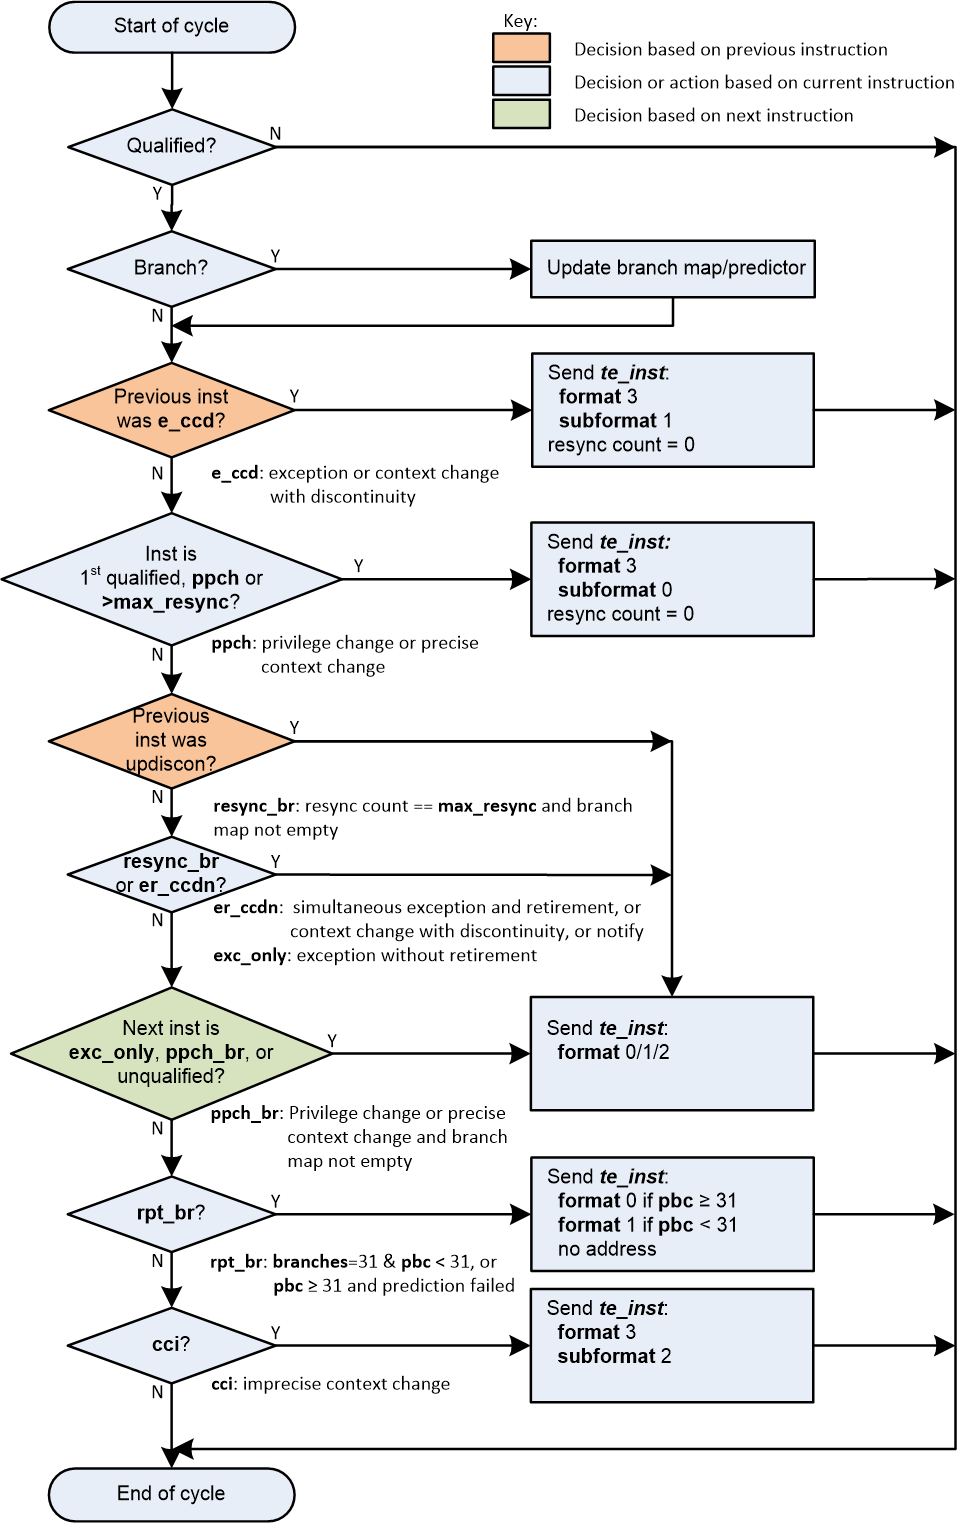
\includegraphics[height=23cm, width=15cm]{algo.png}
  \caption{Delta Mode 1 instruction trace algorithm}
  \label{fig:algo}
\end{center}
\end{figure}

Figure~\ref{fig:algo} shows instruction by instruction behavior, as would be
seen in a single-retirement system only.  Whilst the ingress port allows the RISC-V core to
provide information on multiple retiring instructions simultaneously, the resultant packet
sequence generated by the encoder must be the same as if retiring one instruction at a time.

A 3-stage pipeline is assumed, such that the encoder has 
visibility of the current, previous and next instructions.  All packets are generated using 
information relating to the current instruction.  The orange diamonds indicate decisions 
based on the previous (or last) instruction, the green diamond indicates a decision based on the
next instruction, and all other diamonds are based on the current instruction.

Additionally, the encoder can generate one further packet type, not shown on the diagram for 
clarity.  The \textit{support} packet (format 3, subformat 3 - see Chapter~\ref{packets}) is 
sent when:

\begin{itemize}
  \item The encoder is enabled or disabled, or its configuration is changed, 
    to inform the decoder of the operating mode of the encoder
  \item After the last qualified instruction has been traced, to inform the decoder that 
    tracing has stopped;
  \item If trace packets are lost (for example if the buffer into which packets are being 
    written fills up.  In this situation, the 1st packet 
    loaded into the buffer when space next becomes available should be a \textit{support} 
    packet.  Following this, tracing will resume with a sync packet.
\end{itemize}

Note: if the \textbf{halted} or \textbf{reset} sideband signals are asserted (see Table~\ref{tab:ingress-side-band})
the encoder will behave as if it has received an unqualified instruction (output \textit{te\_inst}
reporting the address of the last instruction, followed by \textit{te\_support});


\section{Full vs Differential Addresses} \label{addresses}
Addresses can be output in one of two ways: \textit{full} or \textit{differential}.

\begin{itemize}
  \item The \textit{full} address is the actual address of the current instruction;
  \item The \textit{differential} address is the difference between the actual address of 
    the current instruction and the actual address of the instruction reported in the 
    previous packet that contained an address.
\end{itemize}

Packet formats 1 and 2 include a differential address, whilst format 3 includes the full address.

If the optional full address mode is enabled (see Section~\ref{sec:full-address}), all packet formats
will include a full address.

\section{Format selection} \label{format-selection}

In all cases but one, the packet format is determined only by a 'yes' outcome from the 
associated decision.  The choice between formats 1 or 2 for the case in the middle of the 
diagram needs further explanation.  

If there are no branches that need to be reported, packet format 2 is used.  

If there are branches to report, format 1 is used.

If branch prediction is supported and is enabled, then there is a choice of whether to output a 
full branch map, or a count of correctly predicted branches.  In order to choose the count, the number 
of correctly predicted branches must be at least 31.  If there are 31 unreported branches (i.e. the branch
map is full), but not all of them were predicted correctly, then the branch map will be output.
If all 31 unreported branches were correctly predicted, then the encoder starts counting
subsequent correct predictions, and will output a count under the following conditions:

\begin{itemize}
  \item A branch is mis-predicted.  The count value will be the number of correctly predicted branches, 
    minus 31.  \textbf{branch\_fmt} will be 01, indicating that the next branch failed its prediction.
   No address information is provided;
  \item An updiscon, interrupt or exception requires the encoder to output an address.  In this case 
    the encoder will output the branch count (number of correctly predicted branches, minus 31) with 
    \textbf{branch\_fmt} set to 10.  The packet also contains \textbf{mispred}, indicating whether 
    prediction of the next branch failed.
  \item The branch count reaches its maximum value (0xffff).  Again, \textbf{branch\_fmt} will be set to 10.
    Strictly speaking an address isn't required for this case, but it will occur so rarely that the bandwidth 
    impact can be ignored
\end{itemize}

Packet formats 1 and 2 are organized so that the address is usually the final field.  Minimizing the 
number of bits required to represent the address reduces the total packet size and significantly
improves efficiency.  See Chapter~\ref{packets}.

\section{Resynchronisation} \label{sec:resync}

Per Section~\ref{synchronization}, a format 3 synchronisation packet must be output after "a prolonged
period of time". The exact mechanism for
determining this is not specified, but options might be to count the number of \textit{te\_inst} packets emitted, 
or the number of clock cycles elapsed, since the last synchronization message was sent.

When the resync is required, the primary objective is to output a format 3 packet, so that the decoder can 
start tracing from that point without needing any of the history.  However, if the decoder is already synced, 
then it is also required that it can continue to follow the execution path up to and through the format 3 packet 
seamlessly.  As such, before outputting a format 3 packet, it is necessary to output a format 1 packet for the 
preceding instruction if there are any unreported branches (because format 3 does not contain a branch map).  
The format 3 will be sent if the resync timer has been exceeded.  On the cycle before this (when the resync timer 
value has been exactly reached), a format 1 will be generated if the branch map is not empty.
